\documentclass{elbioimp2}
\usepackage[utf8]{inputenc}

\usepackage[backend=biber,style=vancouver]{biblatex}
\usepackage{csquotes}
\usepackage[braket]{qcircuit}
\usepackage{float}

\title{The state of Quantum Computing in 2025}
\shorttitle{The state of Quantum Computing in 2025}
\author{Adam Prior.\affiliation{UrbanFox, Dublin, Ireland}} 
\shortauthor{A. Prior.}
% \elbioimpreceived{19 Sept 2025}  
% \elbioimppublished{19 Sept 2025}
% \elbioimpfirstpage{1}
% \elbioimpvolume{x}
% \elbioimpyear{20xx}
 
\addbibresource{bibliography.bib}

\begin{document}
\setcounter{secnumdepth}{2}


\maketitle

\begin{abstract}
This paper provides an accessible overview of the current state of quantum computing technologies as of September 2025. Aimed at readers with a technical background but no prior experience in quantum computing, this paper reviews foundational concepts, historical advancements, and leading hardware and software platforms. The paper also discusses practical challenges, potential applications, and the outlook for future developments in the field.

  \keywords{Quantum Computing; Qubits; Decoherence; robotics}
\end{abstract}

\section{. Introduction}
Define Quantum Advantage here.
Define Some other terms here.


\section{. Historical Advancements in Quantum Computing}
The first mentions of quantum computation can be traced as far back as the early as 1980s.
In 1980, mathematician Yuri Manin discussed the concept of a quantum computer in his book \textit{Computable and Non Computable}\cite{Manin1980}. Richard Feynman, in 1982, published a paper

`Simulating physics with computers', introducing the idea of simulating quantum systems using quantum computers\cite{Feynman1982}. Feynman highlighted the limitations of classical computers in simulating the exponentially growing state space of quantum systems, and how quantum computers could perform these simulations more efficiently.


Following these initial years of foundational work, the field began to gain traction, leading to another \textit{10 years} of significant theoretical developments. In 1985, David Deutsch advanced quantum computing theory by rigorously defining the Universal Quantum Turing Machine—the quantum analog of a classical Turing machine—capable of performing any computation that a classical computer can, but more efficiently for certain problems\cite{Deutsch1985}.
Further theoretical progress included contributions such as reversible quantum computation by Paul Benioff between 1985 and 1987\cite{benioff1986}, the first proposal of a physically realizable quantum computer using atoms and photons in 1998\cite{Igeta:88}, and attempts to define quantum complexity classes in 1989\cite{10.1145/167088.167097}. These efforts eventually led to the definition of Bounded-Error Quantum Polynomial Time (BQP) problems, an important class in complexity theory that can be efficiently solved by quantum computers in polynomial time.

It was not until 1992 that the first quantum algorithm was proposed by Deutsch and Jozsa\cite{Deutsch1992RapidSO},
demonstrating that quantum computers could solve certain problems more efficiently than classical computers 
(quantum advantage). While this algorithm has very limited practical applications, it paved the way for more 
impactful algorithms.
The most famous of these is Shor's algorithm, proposed by Peter Shor in 1994\cite{365700}. Shor's algorithm 
is an efficient quantum algorithm for integer factorization in polynomial time, versus the best known classical
algorithms which run in sub exponential time. This algoirithm in some sense `proved' the potential of quantum computing
to solve practical problems that are intractable for classical computers, particularly in the context of cryptography, as
many encryption schemes rely on the difficulty of factoring large integers. 
Another significant algorithm is Grover's algorithm, proposed by Lov Grover two years later\cite{grover1996fastquantummechanicalalgorithm}, providing
quadratic speedup for unstructured search problems.

While these algorithms demonstrate the theoretical potential of quantum computers, they would be useless without

the ability to assemble a physical quantum computer. Around the same time as these algorithmic developments, experimental researchers were developing the first real qubits and quantum gates. The first experimental demonstration of a quantum logic gate was realized in 1995 by a team using an electromagnetic trap to confine ions in place, forming a two-qubit system. The energy levels of the ions were used to represent the qubit states (|0⟩ and |1⟩), while laser pulses manipulated these states. The team successfully implemented a controlled-NOT (CNOT) gate, a fundamental universal quantum gate used in many quantum algorithms\cite{PhysRevLett.75.4714}.
This point in time can be considered the take-off moment in the history of quantum computing, as it was demonstrated—roughly in parallel—to be both theoretically computationally advantageous (for certain classes of problems) and experimentally realizable. A large acceleration in research and development followed. Over the next decade, experiments demonstrated more complex gates and increased numbers of qubits (8-qubit registers by December 2005)\cite{8bitregister}, as well as new quantum systems capable of implementing qubits, such as superconducting states, nuclear spins, quantum dots, and even photon polarization. Theoretical advancements also continued, with the development of quantum error correction codes and various proofs of principle for quantum algorithms that further highlighted feasibility and limitations.


Up to this point, it is well known that quantum computers suffer from extreme scaling problems. Qubits are highly sensitive to their environment and are severely affected by quantum decoherence, which limits the rate at which additional qubits can be added to a system before the entire system becomes unstable. This sensitivity explains why it took so long to scale beyond only a few qubits. Table~\ref{tab:qubit_counts} summarizes some of the key leaps in qubit counts over the years.

\section{. Fundamentals of Quantum Computing}
In order to properly understand the current state of quantum computing, it is important to first understand
some of the fundamental concepts. What exactly is a qubit? What is superposition and entanglement? What is a quantum gate?

\subsection{. Qubits and their construction}
For the average reader without a background in quantum mechanics, but with some technical background in computing, a qubit can be thought of as the quantum analog of a classical bit. When we use the term `classical', we specifically mean non-quantum, referring to the type of computing that underpins all modern computers today. A classical bit represents the fundamental unit of information in classical computing and is binary in nature, meaning it exists in one of two states, usually represented as 0 or 1. In classical physics, it is straightforward to encode a bit's state as either 0 or 1, typically using voltage levels, where a high voltage might represent a 1 and a low voltage a 0. An important point to note is that a classical bit can only exist in one of these two states at any given time. In classical physics, there is no such thing as being both high and low voltage simultaneously; it is always one or the other.

Similarly, a qubit is also a binary unit of information, but it operates according to the principles of quantum mechanics. Many quantum mechanical systems can be used to physically realize a qubit, and in general, any two-level quantum system can serve as a qubit. For example, the spin angular momentum of an electron can take two distinct values: `up' or `down', which correspond to the 0 and 1 states of a qubit. Other physical systems that can be used to realize qubits include the polarization states of photons, energy levels of atoms or ions, and superconducting circuits. We are not limited to electronic spins alone. A rich variety of physical systems can be used to implement qubits, each with its own advantages and challenges. Such systems include, but are not limited to:
\begin{itemize}
  \item Trapped ions and neutral atoms electronic states
  \item Superconducting states (charge, flux, or phase)
  \item Photonic qubits (polarization states, number of photons, etc)
  \item Quantum dots (electron localization states, spin)
  \item Nuclear spins (nuclear magnetic resonance spin)
\end{itemize}

When we consider that the underlying quantum system is simply being used as an alternative way to encode a binary state, it might be tempting to view a qubit as merely a more complex representation of a classical bit. However, the true power of qubits lies in their ability to exist in a state called \textit{quantum superposition}, which is a fundamental principle of quantum mechanics.


\subsection{. Quantum States, Superposition and Entanglement}
In quantum mechanics, we represent the state of a quantum system using a special notation called bra-ket notation. In this notation, the up state is represented as $|0\rangle$ and the down state as $|1\rangle$. As mentioned previously, however, unlike a classical bit, a qubit can exist in a combination (superposition) of both states simultaneously. For those who are mathematically inclined, this means that a qubit can be in a state that is a linear combination of $|0\rangle$ and $|1\rangle$, represented mathematically as:
\begin{equation}
  |\psi\rangle = \alpha|0\rangle + \beta|1\rangle
\end{equation}

where $\psi$ just means `the state of the qubit'. The coefficients $\alpha$ and $\beta$ are complex numbers that represent the probability amplitudes of the qubit being in the $|0\rangle$ and $|1\rangle$ states, respectively. This expression for the superposition, given that the complex coefficients are continuous values, shows us that the qubit has an uncountably infinite number of possible states, with a state for every possible combination of $\alpha$ and $\beta$. This is in stark contrast to a classical bit, which can only be in one of two discrete states.
\begin{figure}[htbp]
  \centering
  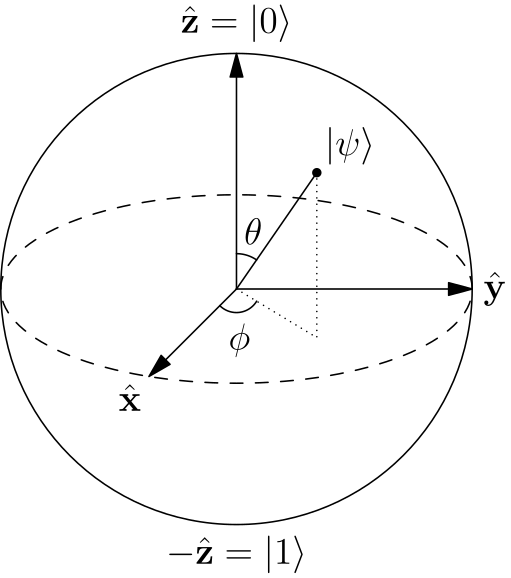
\includegraphics[width=0.75\columnwidth]{assets/bloch-sphere.png}
  \caption{The Bloch Sphere representation of a qubit. Any point on the surface of the sphere represents a valid qubit state, with |0⟩ and |1⟩ at the poles. The angles $\theta$ and $\phi$ determine the specific superposition state.}\label{fig:bloch-sphere}
\end{figure}

The probabilities of measuring the qubit in either state are given by the squares of the magnitudes of these coefficients. In some sense, they represent the `weight' of each state in the superposition—the likelihood that measuring the qubit will yield that particular state. In quantum mechanics, the act of measurement causes the qubit to `collapse' into one of the base states (either |0⟩ or |1⟩), with probabilities determined by these coefficients. It is this superposition that enables quantum computers to perform certain computations more efficiently than classical computers, as these complex coefficients can interfere constructively or destructively during quantum computations, allowing quantum algorithms to amplify the probabilities of correct answers while suppressing incorrect ones.

The nature of superposition also leads to the concept of \textit{entanglement}, another fundamental property of quantum mechanics. When two qubits become entangled, the state of one qubit becomes directly correlated to the state of the other, regardless of the distance between them. This means that measuring one qubit instantly determines the state of the other. Entanglement is a key resource in many quantum algorithms and protocols, enabling phenomena such as quantum teleportation and superdense coding. It is also a crucial component in achieving quantum advantage, as it allows for correlations that are not possible in classical systems; there is no classical analog to entanglement. It is a purely quantum mechanical phenomenon.

As the coefficients $\alpha$ and $\beta$ are complex numbers, they have both a magnitude and a phase, and it is this phase that allows for interference effects to occur due to relative phase differences between qubit states. Maintaining stable relative phases is critical for the proper functioning of quantum algorithms, and is measured by a property called coherence time, which is the time over which a qubit can maintain its quantum state before loss of information to the environment (decoherence) occurs. The global coherence of a multi-qubit system is particularly important, as quantum algorithms often rely on the interference of amplitudes across multiple qubits to achieve their computational advantage. Two important metrics used to quantify the coherence of qubits are $\tau_1$ and $\tau_2$ times. $\tau_1$, or relaxation time, measures how long a qubit can stay in an excited state before it decays to its ground state due to energy loss to the environment. $\tau_2$, or dephasing time, measures how long a qubit can maintain its phase coherence before interactions with the environment cause it to lose its quantum information. Both $\tau_1$ and $\tau_2$ times are critical for the performance of quantum computers, as they determine how long quantum information can be reliably stored and manipulated.

\subsection{. Quantum Gates}

It's all well and good to be able to create qubits and understand their properties; however, to perform computations, we need a way to manipulate these qubits through quantum gate operations. Quantum gates are the quantum analogs of classical logic gates. While classical gates operate by flipping or combining bits within their restricted classical space, quantum gates are represented mathematically by matrices acting on the state vectors of qubits, enabling flips, rotations, entanglement, and other transformations within the much larger quantum state space. This is best understood by considering the geometric representation of a qubit on the Bloch sphere (see Figure~\ref{fig:bloch-sphere}), where quantum gates can be visualized as rotations of the qubit's state vector on the sphere.

\begin{figure}[h]
  \centering
  \scalebox{1}{
    \Qcircuit{
      \lstick{\ket{q_1}} & \gate{H} & \ctrl{1} & \gate{S} & \qw \\
      \lstick{\ket{q_2}} & \ctrl{2} & \ctrl{0} & \ctrl{1} & \qw \\
      \lstick{\ket{q_3}} & \qw & \qw & \gate{Y} & \qw \\
      \lstick{\ket{q_4}} & \targ & \gate{X} & \qw & \qw \\
    }
  }
  \caption{Example of a simple 4-qubit quantum circuit. Each horizontal line represents a qubit, and the symbols show basic operations that can be performed on them such as the Hadamard gate (H), controlled NOT gate (CNOT), phase gate (S), Pauli-X gate (X), and Pauli-Y gate (Y).}
\end{figure}


In practice, the experimental implementation of quantum gates depends on the physical system used to realize the qubits. For instance, in superconducting qubits, microwave pulses manipulate the energy levels of the qubits, whereas in trapped ion systems, laser pulses control the internal states of the ions. Common single-qubit gates include the Pauli-X, Y, and Z gates (corresponding to bit-flip and phase-flip operations), as well as the Hadamard gate (which creates superposition). Multi-qubit gates, such as the CNOT (Controlled-NOT) gate, are essential for generating entanglement between qubits and enabling more complex quantum operations. Since gate operations are physical processes, they require a finite amount of time. The time needed to perform a gate operation, known as the gate time $\tau_g$, is a critical parameter in quantum algorithms, as it must be much shorter than the coherence times ($\tau_1$ and $\tau_2$; see practical challenges section).

\begin{table*}[t]
  \centering
  \begin{tabular}{|c|c|l|}
  \hline
  \textbf{Year} & \textbf{Qubit Count} & \textbf{Description} \\
  \hline
  1995 & 2 & First experimental demonstration of a quantum logic gate using trapped ions \\
  \hline
  2001 & 7 & Implementation of Shor's algorithm on a 7 qubit NMR quantum computer \\
  \hline
  2005 & 8 & Demonstration of an 8 qubit register using trapped ions \\
  \hline
  2011 & 5 & D-Wave Systems announced a 512 qubit quantum annealer \\
  \hline
  2016 & 16 & IBM unveiled a 16 qubit superconducting quantum processor \\
  \hline
  2017 & 20 & Google announced a 20 qubit superconducting quantum processor \\
  \hline
  2019 & 53 & Google's Sycamore processor achieved quantum supremacy with 53 qubits \\
  \hline
  2020 & 65 & Honeywell announced a 65 qubit trapped ion quantum computer \\
  \hline
  2021 & 127 & IBM unveiled a 127 qubit superconducting quantum processor \\
  \hline
  2022 & 433 & IonQ announced a 433 qubit trapped ion quantum computer \\
  \hline
  2023 & 1000+ & Various companies announced plans for quantum processors with over 1000 qubits \\
  \hline
  2024 & 2000+ & Continued advancements with processors exceeding 2000 qubits \\
  \hline
  2025 & 5000+ & Leading companies project quantum processors with over 5000 qubits \\
  \hline
  \end{tabular}
  \caption{Key advancements in qubit counts from 1995 to 2025 and their corresponding platforms.}\label{tab:qubit_counts}
\end{table*}

\subsection{. Decoherence, Errors, and Correction}
In an actual quantum computer, we are far from the ideal mathematical situation of qubits being perfectly coherent, noise free, and decoupled from the environment. In practice, the quantum states required are incredibly delicate, generally requiring the system to be supercooled to near absolute zero temperatures and isolated from all external influences. Even so, it is impossible to remove all sources of noise, and as such, the system is subject to decoherence. Decoherence is the process by which a quantum system loses its quantum properties due to interactions with its environment. This can occur through various mechanisms, such as thermal fluctuations, electromagnetic interference, or imperfections in the qubit fabrication process. Decoherence leads to the loss of superposition and entanglement, effectively collapsing the qubit states into classical states and destroying the quantum information they carry. This is not a limitation of hardware alone but a fundamental property of quantum mechanics itself. As stated earlier, the coherence times $\tau_1$ and $\tau_2$ are critical metrics that quantify how long a qubit can maintain its quantum state before decoherence occurs. As we add more qubits to the system, the global coherence of the multi-qubit system becomes exponentially more fragile and susceptible to decoherence, making it increasingly challenging to maintain the quantum information across the entire system. Decoherence ultimately results in the occurrence of errors during quantum computations as the global state collapses unpredictably.

Decoherence is not the only source of error in quantum computations. Quantum gate operations themselves are also subject to imperfections and therefore have some probability of failure. For example, attempting to perform an X gate on a qubit in the $|0\rangle$ state might not always successfully flip it to the $|1\rangle$ state due to imperfections in the control pulses or interactions with the environment during the gate operation. This is known as gate error. Gate fidelity measures how accurately a quantum gate performs the intended operation, and is typically quantified using metrics such as average gate fidelity. As a rule of thumb, gate fidelities above 99\% are generally considered good, but for practical quantum computing, even higher fidelities (e.g., 99.9\% or better) are often required.

To mitigate the effects of decoherence and gate errors, quantum error correction techniques are employed. Error correction involves encoding quantum information across multiple physical qubits to create logical qubits that are more robust against errors. This is typically achieved using quantum error correcting codes, such as the surface code or the Steane code, which can detect and correct certain types of errors without directly measuring the quantum information itself (which would collapse the state). Implementing error correction requires additional qubits and gate operations, increasing the complexity of the quantum computer. The overhead for error correction can be substantial, often requiring an order of magnitude more physical qubits to create a single logical qubit. Nevertheless, error correction is essential for achieving fault tolerant quantum computing, allowing computations to be performed reliably even in the presence of noise and errors.


\section{. Practical Challenges in Quantum Computing}
\subsection{. Decoherence and Noise}
As stated in the previous section, the fragility of quantum states plays a major role in the accuracy of quantum computations. Qubits interact unavoidably with their environments, leading to decoherence that destroys superpositions and entanglement, which are essential for quantum advantage and for reducing the error rates of quantum gates. Minimizing decoherence and noise is one of the biggest challenges in building practical quantum computers. The scaling effect of decoherence and noise is especially problematic as the number of qubits increases, making it exponentially more difficult to maintain coherence across the entire system as we enter the realm of hundreds to thousands of qubits.


\subsection{. Gate Fidelity and Speed}
Given the coherence windows $\tau_1$ and $\tau_2$, these set a hard limit on how many gate operations can be performed before the quantum information is lost. As a real example, in trapped ion systems, which can have exceptionally long coherence times on the order of seconds or longer, single-qubit gate times can be on the order of microseconds, while two-qubit gates can take tens to hundreds of microseconds. For a 50 second coherence time and a 500$\mu s$ gate time, this allows for only 100,000 gate operations before decoherence occurs and destroys the computation. When considering a practical algorithm like Shor's algorithm for integer factorization, this number seems more than enough for the trivial example of factoring the number 15 (4 bits) into its factors of 3 and 5. But entering the regime of RSA encryption, where we are dealing with 2048-bit numbers to be factorized, we are looking at anywhere from billions to trillions of gate operations. Thus, faster gate operations are desirable to maximize the number of operations that can be performed within the coherence time. However, increasing gate speed often comes at the cost of reduced gate fidelity, as faster gates can be more susceptible to control errors and noise. Therefore, a balance must be struck between gate speed and fidelity to optimize the performance of quantum computers.

Gate fidelity itself, an inverse measure of the error rate of a gate operation, is a critical factor, as even tiny errors in gate operations can accumulate over the course of a quantum computation, leading to incorrect results. Achieving high gate fidelities (e.g., above 99.9\%) is essential for practical quantum computing, but this remains a significant challenge due to various sources of noise and imperfections in the control systems used to manipulate qubits. However, we are already approaching and surpassing this threshold, with fidelities exceeding 99.9\% in some platforms such as trapped ions and germanium quantum dots\cite{Srinivas_2021,gemanium999}, and major advancements in 2025 in superconducting qubits have also pushed single gate fidelities reliably beyond 99.997\%\cite{PRXQuantum.5.040342}.

\subsection{. Error Correction, Fault Tolerance and the Logical-Physical Qubit Gap}

Given the probabilistic guarantee of gate faults and decoherence faults, an absolute requirement of quantum computing is to design computations to be fault tolerant. Achieving fault tolerance in quantum computers opens its own entire area of research known as error correction, with its own domain of difficulties. The goal of error correction is to accept that faults are guaranteed to occur, and aims to detect them and, in turn, correct them. In general, this is achieved through the concept of a \textit{logical qubit}.

While actual physical qubits are capable of computation, the probability of error is too high to achieve correct results for realistic problems. A logical qubit is a collection of qubits that are used for redundancy in the case of errors. We might then say that one \textit{useful} qubit consists of multiple physical qubits. It is this logical qubit that quantum computation is done with. The logical qubit becomes a fault tolerant qubit via the implementation of error correction codes, which use the ensemble to correct errors that occur in the logical qubit.

Many different error correction schemes exist, but leading schemes like surface codes or color codes require many physical qubits per logical qubit, leading to a huge overhead in the number of qubits required for practical quantum computing. In 2023, researchers at Google showed experimentally that error rates could be reduced by using increased physical qubit counts\cite{GoogleQAI2023}. Specifically, they showed that increasing the physical qubit count from 17 to 49 per logical qubit, the error rate decreased from 3.0\% to 2.9\%. While this important result shows the potential for improving error rates through increased qubit counts, it also highlights the scale at which we might need to reach to achieve robust error correction. Some modern error correction scheme estimates suggest that practical computing would require hundreds to thousands of physical qubits per logical qubit, requiring a total number of physical qubits in the order of millions for a practical computation. This is often referred to as the logical-to-physical qubit gap, and it represents one of the biggest challenges in scaling up quantum computers to the sizes needed for practical applications. However, only in the last couple of years, huge strides have been made in developing super efficient error correction codes. 2024 research by IBM reported the implementation of a new error correction code called the Gr\"oss code, which protected 12 logical qubits using only 288 physical qubits (24 qubits per logical qubit) for approximately one million error correction cycles, demonstrating a significant reduction in the logical-to-physical qubit ratio\cite{FTQM2024} compared to other leading codes like surface code. Surface code, according to the IBM analysis, would require almost 3000 physical qubits to achieve the same task.

Microsoft and Quintinium, also in 2024, announced similar low ratio logical qubits using only 30 physical to encode 4 logical qubits (7.5 physical per logical qubit) using their own error correction techniques. However, their quantum system is limited to only 32 physical qubits, so while the ratio is impressive, the absolute number of logical qubits is still very small\cite{paetznick2024demonstrationlogicalqubitsrepeated}. However, this highlights the rapid pace of advancements in error correction codes and the potential for more efficient schemes to significantly reduce the overhead required for fault tolerant quantum computing.

While these results are promising, it is important to note that these are still early days in the development of practical error correction codes, and much work remains to be done to fully understand their performance and scalability in real world quantum computing systems.

\subsection{. Time \& Space resource requirements for practical algorithms}
The particularly well-known Shor’s algorithm is regularly used as the benchmark for quantum computing, as it is one of the most famous algorithms that demonstrates a clear quantum advantage over classical algorithms. It has been suggested in simpler implementations that Shor's algorithm for factoring an $n$-bit integer can be achieved with as few as $2n+3$ \textit{logical} qubits, with the number of gate operations required to achieve the factorization scaling as $O(n^3)$\cite{beauregard2003circuitshorsalgorithmusing}. Given RSA encryption with 2048-bit integers, this suggests RSA encryption breaking could be done with 4099 logical qubits, but would require tens of billions of gate operations (high gate depth) consisting of modular quantum additions, multiplications, and Fourier transforms generally performed sequentially. Given the current state of gate speeds and coherence times, this is far beyond the capabilities of current quantum computers, as the system would decohere long before the computation could complete.

Further research has investigated trading space for time and vice versa, that is, using circuits that require more qubits to reduce the overall gate depth, or circuits that use fewer qubits but require more gate operations. However, even with these optimizations, the resource requirements for practical implementations of Shor's algorithm remain extremely high. More recent estimates suggest that factoring a 2048-bit integer using Shor's algorithm would require on the order of 20 million physical qubits when considering error correction overheads and realistic gate fidelities, in a computation taking around 8 hours\cite{Gidney_2021}. However, no quantum computer with this physical qubit count is anywhere close to being built. On the flip side, trading time for space to minimize qubit counts, a 2024 paper proposed a method to factor a 2048-bit integer using only $n/2$ logical qubits (roughly 1024 logical qubits), but at the cost of an extremely high gate depth requiring on the order of tens of trillions of operations\cite{10.1007/978-3-032-01878-6_13}. Even with optimistic gate speeds of 1 microsecond per gate and perfect error correction, this computation would take around 230 days to complete.

Considering the largest quantum computers to date, attention is generally brought to D-Wave's Advantage system, which boasts 5000+ qubits\cite{NatureQC2023}. However, this does not actually operate as a universal quantum computer, as it is specifically designed for optimization problems using quantum annealing. Despite this limitation, it highlights the vast discrepancy between current qubit counts and the requirements of millions for practical applications like breaking RSA encryption.


\subsection{. Qubit Connectivity, Control, and Engineering Challenges}

As quantum computers scale up, several engineering challenges emerge that impact their and scalability.

The physical layout of qubits is dictated by the underlying technology. Whether it's superconducting circuits, trapped ions, neutral atoms, or spin qubits each impose specific geometrical constraints on how qubits can interact. Most current platforms support only nearest neighbor connectivity, limiting the ability to perform entangling operations between distant qubits. While research into long range entanglement and modular interconnects is ongoing, practical quantum networks remain immature. As qubit density increases, cross talk becomes a significant issue, where imperfect isolation, physical proximity, and electromagnetic interference, amogst other effects can couple interactions across the system, degrading overall fidelity and thus increasing the likelihood of errors occuring.

Each qubit in a quantum processor requires precise calibration of its operating parameters, including laser frequencies, pulse shapes, and error mitigation settings. This complexity grows rapidly with the number of qubits, leading to a “complexity explosion” in control systems. The control systems required such as laser sources, and cryogenic infrastructure scale poorly in terms of energy consumption and system complexity. Additionally, hardware drift and environmental fluctuations necessitate frequent recalibration, reducing system uptime and computational efficiency.

The physical requirements for operating quantum hardware are extreme. Superconducting qubits, for example, require dilution refrigerators operating at temperatures near 10 mK, which are difficult to scale to support millions of control lines. Trapped ion and neutral atom systems depend on stable laser and vacuum setups, which are challenging to miniaturize and integrate. Fabrication of quantum devices also presents major hurdles: achieving uniform, and reproducible high fidelity qubits is an open challenge, with device variability causing significant error rates.

Together, these challenges necessitate the need for advances not only in quantum theory and algorithms, but also in engineering, materials science, and systems integration to realize quantum computation at scale.


\section{. Leading Quantum Hardware Platforms}
\subsection{. Superconducting Qubits}
Superconducting qubits are among the most widely used platforms for quantum computing, leveraging Josephson junctions to create two-level quantum systems. These qubits are fabricated using standard microfabrication techniques and operate at millikelvin temperatures using dilution refrigerators. Superconducting qubits offer fast gate speeds and are highly scalable, with leading implementations from IBM, Google, and Rigetti. Google have claimed quantum supremacy with their Sycamore processor with a count of 53 physical qubits in 2019 though this claim has sparked debate due to the benchmarking used. Similarly the more modern 105 qubit google quantum processor, Sycamore, has been developed, with claims of `below threshold' error corrections, though demonstrations are limited to specific cases\cite{google2025}. IBM also have notable quantum processors, with their Heron r2 and condor processors, having 156 and 1121 superconducting qubits. While condor has nearly an order of magnitude more qubits, the Heron r2 has higher fidelities and lower error rates, highlighting the trade offs between qubit count and quality, when compared in actual benchmarking tests\cite{postquantum2024}.

\subsection{. Trapped Ions}
Trapped ion quantum computers use electromagnetic fields to confine ions in vacuum chambers, with qubit states encoded in the internal energy levels of the ions. Laser pulses are used to manipulate and entangle the ions, achieving high-fidelity gate operations and long coherence times. Companies like IonQ and Honeywell have demonstrated significant advances in scaling trapped ion systems. The main challenges are slow gate speeds and difficulties in miniaturizing the control hardware. Quantinuum have  anounced a 96 qubit trapped ion system to be accessible via Hardware-as-a-service in 2025\cite{quantinuum2025} with 99.9\% fidelity in both one and two-qubit gates across all qubit pairs with all-to-all connectivity across qubits They also claim around 50 logical quibits are possible. IONQ have a similar 36 qubit system with high fidelities and expect to increase to 64 qubits in 2025\cite{IonQ2025}.

\subsection{. Photonic Qubits}
Photonic quantum computers encode qubits in the polarization, path, or number states of photons. These systems operate at room temperature and are naturally immune to many noise sources such as charge, flux and magnetic fields due to photons themselves being uncharged. Photonic platforms are well-suited for quantum communication and networking, with companies like Xanadu and PsiQuantum leading development. Challenges include efficient photon generation, detection, and scalable entanglement. However photonic systems lag behind other platforms in terms of qubit counts and gate fidelities, with current systems typically limited to tens of qubits.

\subsection{. Neutral Atoms}
Neutral atom quantum computers trap individual atoms using optical tweezers, encoding qubits in atomic energy levels. These systems offer flexible connectivity, due to the configurable tweezers allowing for more complex atom arrangements, and long coherence times, with companies like Atom, QuEra and ColdQuanta making progress in scaling up atom arrays. Challenges include precise control of atom positions and maintaining stability over large systems. Atom computing's flagship system, AC1000, has 1225 qubit sites, with 1180 high fidelity physical qubits actually implemented\cite{atom2023}.

\subsection{. Quantum Annealers}
Quantum annealing devices, such as those developed by D-Wave, use large arrays of qubits to solve optimization problems by evolving the system toward a ground state. In 2020, D-wave announced a 'commercial' 5000+ qubit quantum annealer built on superconducting qubits, and later a 4400 qubit annealer with much higher performance\cite{DWave2024} While quantum annealers do not act as universal quantum computers, they have demonstrated practical applications in optimization problems. The fact that they do not oeprate as a universal quantum computer allows for much lower fidelity limitations due to the system not being gate based and ultimtely not requiring high coherence, which allows annealers to scale to much higher qubit counts than leading companies largest universal gate based systems. Limitations include restricted problem types and lack of universal gate operations.

\subsection{. Majorana Qubits}
While not a leading platform, Majorana Quasiparticle qubits are a type of topological qubit that leverage non-abelian anyons to achieve fault tolerance. These qubits are expected to be much more robust against local noise due to topological protection, making them promising candidates for scalable quantum computing. Companies like Microsoft are actively researching Majorana qubits, with the goal of creating a topological quantum computer that can operate at higher temperatures and with greater stability than traditional qubit systems. However, Majorana qubits are still in the experimental stage, with many technical challenges to overcome before they can be used in practical quantum computers. It is not yet proven whether Majorana quibits can actually be used to create a functional qubit, with other researchers disputing their usefulness due to previously unexplored mechanisms of decoherence\cite{alase2025decoherencemajoranaqubits1f}. Microsoft however remains optimistic about the potential of Majorana qubits, and continues to invest in research and development in this area.

\section{. Applications}
Quantum computers are not general purpose accelerators; their promise lies in domains where the structure of the problem aligns with quantum mechanical principles such as superposition, entanglement, and interference. Below are the leading application areas, each motivated by the type of computational hardness they address.

\subsection{. Quantum Simulation and Molecular Modeling}
Quantum systems are inherently difficult for classical computers to simulate, since the Hilbert space of an N-particle system grows exponentially with N. Quantum computers can directly map molecular Hamiltonians to qubit registers. Applications include, but are not limited to, drug discovery and protein ligand binding studies, catalysis and industrial chemistry (e.g. nitrogen fixation, battery materials), high-temperature superconductivity and correlated electron systems, and even material discovery. Proof of concept simulations for small molecules ($H_2$, LiH, Fe–S clusters) have been performed on noisy intermediate scale qubit (NISQ) devices. Fault-tolerant devices on the order of tens of thousand logical qubits will be required for chemically relevant systems.

\subsection{. Optimization Problems}
Many industrial problems reduce to combinatorial optimization (scheduling, routing, supply chain). These are NP-hard, with solution spaces that grow exponentially with size. Quantum algorithms such as the Quantum Approximate Optimization Algorithm (QAOA) or quantum annealing aim to find low-energy configurations efficiently. Application include logistics optimization for airlines, shipping, and manufacturing, portfolio optimization in finance, power grid balancing and traffic flow optimization and more.

\subsection{. Cryptography \& Security}
Quantum computing has profound implications for cryptography and information security. The most notable impact arises from quantum algorithms that threaten the security of widely used classical cryptosystems.

Shor’s algorithm enables efficient factorization of large integers and computation of discrete logarithms in polynomial time on a quantum computer. This capability directly compromises the security of RSA and Elliptic Curve Cryptography (ECC), both of which rely on the classical computational hardness of these problems. In contrast, Grover’s algorithm provides a quadratic speedup for brute-force search problems, reducing the search complexity quadratically. While this does not break symmetric cryptographic systems outright, it effectively halves their key strength, necessitating longer keys for equivalent security. It should be reiterated though that we are still far from having quantum computers capable of running these algorithms at the scale required to break practical cryptographic systems.

Once fault-tolerant quantum computers with sufficient qubit counts are realized, Shor’s algorithm could be used to break RSA, ECC, and other public-key schemes, exposing encrypted data and secure communications.
However, the looming threat of quantum attacks has driven the development of post-quantum cryptographic standards, focusing on algorithms (e.g., lattice-based, code-based) believed to be resistant to quantum attacks. Quantum mechanics also enables protocols for provably secure communication, such as quantum key distribution (QKD), which leverages quantum states to detect eavesdropping and guarantee secrecy.

\subsection{. Quantum Communication and Networking}
Photons are natural “flying qubits”, a property which, along with entanglement, can enable secure communication, and connected distant quantum processors in distributed quantum architectures. Active research areas include quantum repeaters to extend communication distances, quantum internet protocols, and integration with classical networks. QKD would likely be implemented in this domain.

\subsection{. Machine Learning \& AI Integration}
Quantum computers can, in principle, accelerate linear algebra routines (matrix inversion, kernel evaluation) at the core of many machine learning models. Quantum feature spaces also allow representation of data that may be intractable classically. Applications in this area are still exploratory, but include quantum-enhanced classifiers, generative models, and reinforcement learning. Hybrid quantum-classical architectures are likely to be the first practical implementations. A literature review of quantum machine learning will be presented in a future work.

\section{. Future Outlook \& Roadmaps}
Leading technology companies and research institutions have published roadmaps outlining their visions for the development of quantum computing over the next decade and beyond. These roadmaps typically include milestones for qubit counts, gate fidelities, error correction capabilities, and application demonstrations, with unique roadmaps for each quantum hardware platform, as each platform has its own strengths, weaknesses, and scaling challenges.

For superconducting qubits, companies like IBM and Google have set ambitious goals for scaling up their qubit counts while improving gate fidelities. IBM's roadmap envisions reaching 100 million gate operations on 200 qubits in the near term, with plans to demonstrate error corrected logical qubits within the next few years. Google's roadmap focuses on achieving quantum advantage for specific applications, such as quantum chemistry simulations, while also working towards fault tolerant quantum computing.

IonQ's more recent roadmap (June 2025) for trapped ion qubit systems emphasizes scalability through modular architectures, aiming to connect multiple ion traps to create larger quantum processors. They also plan to improve gate speeds and fidelities to enable more complex algorithms. Their goal is by 2028 to have developed single quantum processors with 10,000 physical qubits and demonstrate a two-chip interconnect for a total system size of 20,000 qubits\cite{ionq2025}, and by 2030 to use this rapidly scaling architecture to produce a system entering a regime of over 20 million qubits.

An up to date (August 2025) roadmap summary of the major players in quantum computing is given by Quantum Insider\cite{quantuminsider2025}. The summary of the roadmaps shows very promising, if not optimistic, near term goals of reaching various different milestones, from aiming for large qubit counts, to smaller but highly fault tolerant logical qubit systems. However, it is important to note that these roadmaps are projections based on current understanding and technology trends, and the actual pace of progress may will likely due to unforeseen technical challenges or breakthroughs.

\section{. Conclusion}
While we are still a long way from building large scale, fault tolerant quantum computers capable of solving practical problems beyond the reach of classical computers, significant progress has been made in recent years. Advances in qubit technologies, error correction codes, and quantum algorithms have brought us closer to realizing the potential of quantum computing. We have already entered the era of Noisy Intermediate Scale Quantum (NISQ) devices, which, despite their limitations, provide valuable platforms for exploring quantum algorithms and applications. Quantum Hardware-as-a-Service (QHaaS) models are making quantum computing more accessible to researchers and developers via the cloud from companies like AWS, which fosters smaller scale innovation and experimentation in the field without the need for vast capital to invest in hardware. 

With huge players like IBM, Google, Microsoft, Intel, and various startups investing heavily in quantum research and development, the pace of innovation is accelerating. Collaborative efforts between academia, industry, and government agencies are driving advancements across multiple fronts, from fundamental physics to engineering and software development.

However, many challenges remain, including improving qubit coherence times, gate fidelities, and scaling up qubit counts while managing complexity and control. Continued research and development across multiple disciplines will be essential to overcome these hurdles and unlock the transformative capabilities of quantum computing at scale.

\newpage

\nocite{*}

\printbibliography[heading=bibintoc,title={References}]

\end{document}
